\scanpage{32}
% archive foliation: 31
un \uline{ensemble} $T(F_1,-,F_n)$ de \deleted{des} faisceaux \inserted{cohérents} sur $X$, de façon que
\margin{à \unsure{généraliser}}

(i) Si les $F_i$ sont remplacés par des $F'_i$ isomorphes, \inserted{tout faisceau $\in$} $T(F'_1,-F'_{\unsure{i|n}})$ est isom. à \deleted{\unsure{$T$}} un faisceau $\in T(F_1,-F_n)$

(ii) Compatibilité avec l'extension de la base : $T(F_1\otimes k',-F_n\otimes k')$ est (à isomorphisme près) l'ens des faisceaux $G\otimes k'$, où $G\in T(F_1,-,F_n)$.
\figure{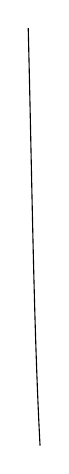
\begin{tikzpicture}\draw (0,0)..controls (.05,-2) and (.07,-3.8)..(.15,-5.3);\end{tikzpicture}}

\uline{Déf 4} Si alors $A_i$ est une partie de $\unsure{\Phi|\mathrm{Cl}}(X/k)$, $(i=1,\ldots,n)$ on désignera par $\Phi(A_1,-A_n)$ l'ens des classes \inserted{de $\unsure{\Phi|\mathrm{Cl}}(X/k)$} des él. des $\Phi(F_1,-F_n)$, où $F$ est cohérent sur $\widetilde X$ et $\operatorname{cl}_k(F_i)\in A_i$ pour tt $i$.
\figure{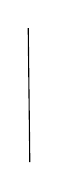
\begin{tikzpicture}\draw (0,0)--(.02,-1.7);\end{tikzpicture}}
\margin{\unsure{introduire} la \unsure{prop.} et la définition}

On voit \deleted{de \unsure{suite}}\inserted{facilement} que la définition ne change pas si on remplace $\widetilde k$ par une extension $\widetilde k'$ de $\widetilde k$ ayant les mêmes propriétés, et il est d'ailleurs facile de donner une définition directe de $\Phi(A_1,-A_n)$ sans utiliser $\widetilde k$, comme l'ens des classes
\margin{\unsure{proposition} 5}
